\documentclass[reprint, amsmath, amssymb, aps]{revtex4-2}

\usepackage{graphicx}% Include figure files
\usepackage{dcolumn}% Align table columns on decimal point
\usepackage{bm}% bold math
\usepackage[inline]{enumitem}  

\newcommand{\that}[1]{\widetilde{#1}}


\begin{document}




\title{A Review on the Rydberg CNOT Gate \\and the Application of Floquet Theory in Studying Two-level Systems}

\author{Jinyan Miao}
 \email{jmiu@umich.edu}
\affiliation{Department of Physics, University of Michigan, Ann Arbor, MI 48109, USA}
\hfill\break
\date{\today}


\begin{abstract}
We present a review of the mechanism of building the Rydberg CNOT gate, which based mostly on the study of two-level systems in the semi-classical approach and the Rydberg blockade in Rydberg atoms. Then we extend our studies on two-level systems by considering the temporal periodicity in the Hamiltonian; we discuss the application of Floquet theory and its spatial analogue Bloch theory, in studying the periodicity in the Hamiltonian; and finally, we examine the utilization of Floquet engineering in investigating optical lattices.
\end{abstract}

\maketitle

\section{\label{sec:level1}Introduction}
As any unitary operation on states in quantum computers can be obtained using a complete set of universal gates, experimentally building the universal gates has been one of the main research interests in quantum physics. One example of a complete set of gates consists of single qubit operations and a two-qubit controlled-NOT (CNOT) gate. The CNOT gate has been demonstrated in
several different physical systems including trapped ions \cite{2, 3}, superconducting circuits \cite{4,5}, and linear optics \cite{6,7}. Numerous proposals exist for neutral atom quantum
gates including short range dipolar interactions \cite{8}, ground state collisions \cite{9}, coupling of atoms to photons \cite{10}, magnetic dipole-dipole interactions \cite{11}, gates with delocalized qubits \cite{12}, and the one that we will discuss in this text, Rydberg state mediated dipolar interactions \cite{13, Isenhower, IsenhowerThesis}. On the theoretical side, the use of the two-level system model in describing an atom interacting with an external field has been a crucial component in constructing the CNOT gate in many approaches. The first part of this text dedicates to discuss the working mechanism of the Rydberg CNOT gate, starting with the two-level model in the semi-classical approach, the Rydberg blockade due to the dipolar interactions between the Rydberg atoms, and the combination of the two to build the Rydberg CNOT gate. \\


In the second part of the text, we will continue our discussion on the two-level system model.
When addressing two-level system problems, the rotating-wave approximation (RWA) has been widely employed to simplify the calculation, while it is effective only under the condition where the Rabi frequency is much smaller than the transition frequency. In the cases where RWA is inapplicable, a common approach is to employ the Floquet theory \cite{Shirley, Engelhardt, Wang}. This approach entails expressing the evolution of a system as a Fourier series with respect to the oscillation frequency \cite{Campaioli, Viebahn}. Beyond its application to simple two-level systems in quantum optics, Floquet theory offers a powerful platform for dealing with the time-dependent Schrödinger equation by leveraging any time-periodicity within the Hamiltonian. Its utility extends broadly across various time-dependent scenarios, encompassing areas such as photonic Floquet topological insulators \cite{Rechtsman}, quantum information processing \cite{88}, heat engines and laser cooling \cite{89}, quantum optimal control \cite{90,91}, and time crystals \cite{92,93}. Furthermore, the combination of Floquet theory with its spatially analog, Bloch theory, provides an efficient and rigorous approach to studying optical lattices, which is particularly pivotal in researching the control of cold atom systems \cite{Viebahn, Sandholzer, Anderson}. Thus, in the second part of the text, we will introduce the Floquet theory in describing temporally periodic systems, drawing its parallels with the Bloch theory, and apply it to solve two-level system problems, in both the semi-classical approach and the Jaynes-Cummings model. We will have a closer look at the solutions by solving the two-level system numerically, and discuss why the approach involving the Floquet theory is more efficient. Lastly, we will look at the application of Floquet engineering in studying optical lattices, based on the work by Kilian Sandholzer et al. \cite{Sandholzer}.


\section{\label{sec:level1}A Review On the Two-level System}
For simplicity, we will work in units where $\hbar = 1$. To understand the working mechanism of the Rydberg CNOT gate, we start with a brief review of the two-level system model describing a two-level atom interacting with an oscillating electric field, in the semi-classical approach (where the electric field is not quantized). Here we consider the field to be described by 
\begin{align}
\mathbf{E}(t) = (E_0 e^{-i\omega t} + E_0^*e^{i\omega t})\hat{z}
\end{align}
with angular frequency $\omega$. The total system Hamiltonian can then be written as
\begin{align}
H = H_{\text{a}} + H_{\text{int}}\,,
\end{align}
where
\begin{align}
H_{\text{a}} = \frac{\omega_0}{2}\, \sigma_z 
\end{align}
is the bare Hamiltonian of the two-level atom with $\omega_0$ being the energy separation between the two levels, and 
\begin{align}
H_{\text{int}}  =  (\Omega e^{-i\omega t}+ \that{\Omega} e^{i\omega t} )|1\rangle \langle 0| + (\text{h.c.})
\end{align}
is the interaction Hamiltonian, with $\Omega$ being the Rabi frequency of the two level system, $\that{\Omega}$ being the associated counter-rotating frequency, and $(\text{h.c.})$ meaning the Hermitian conjugate terms. Here $\Omega$ and $\that{\Omega}$ can be calculated via the dipole-dipole interaction between the atom and the field and thus are proportional to the intensity of the field. Combining Eq.\,(2) with the time-dependent Schrodinger equation
\begin{align}
i \frac{\partial}{\partial t}|\psi(t)\rangle = H(t)\, |\psi(t)\rangle\,,
\end{align}
we can solve for the dynamic of the atom described by the state $|\psi(t)\rangle = a_0(t)\,|0\rangle + a_1(t)\, |e\rangle $. The occupation probability of the ground state $|1\rangle$ can then be calculated by $P_0(t) = |a_0(t)|^2$, and similarly for the excited state $|1\rangle$ occupation probability $P_1(t) = |a_1(t)|^2$. \\

\subsection{Rabi flopping}
In the case where $\Omega = \that{\Omega} = \Omega_0$ for some constant $\Omega_0$, one can show \cite{Berman} that the population of the two states of the atom oscillate as a function of time, which is known as the Rabi flopping. In particular, if $a_0(0) = 1$ and $a_1(0) = 0$, we have [Eq.\,(2.92) in \cite{Berman}, Chapter 2] 
\begin{align}
|a_1(t)|^2 = \frac{|\Omega_0|^2}{\Omega'^2} \, \sin^2\left( \frac{\Omega_0 t}{2}\right)\,,
\end{align}
where $\Omega' = \sqrt{\delta^2 + |\Omega_0|^2}$ is the generalized Rabi frequency, and $\delta = \omega - \omega_0$ is the detuning between the field frequency and the separation between the two levels. From here it is straightforward to see that one is able to drive the atom from state $|0\rangle$ to state $|1\rangle$ only when $\delta \approx 0$. That is, to effectively drive the atom between ground and excited states, it is essential to have the field in-resonance with the two-level atom. The numerical simulation of this phenomenon is depicted in Fig.\,1, comparing the case $\delta = 0 $ with the case $\delta = -0.5\omega_0$. 
\begin{figure}
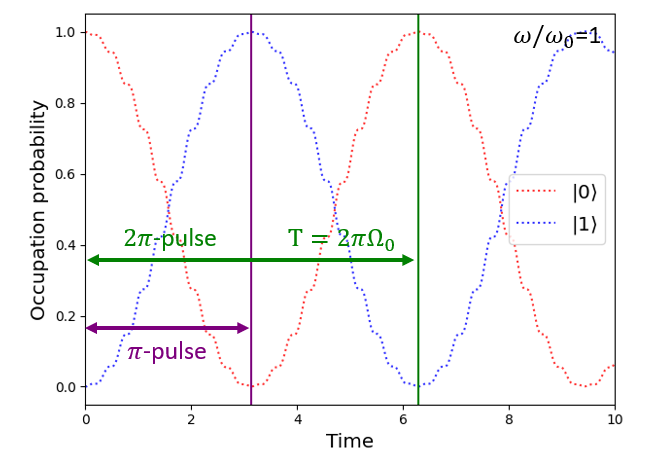
\includegraphics[scale=0.59]{F7}
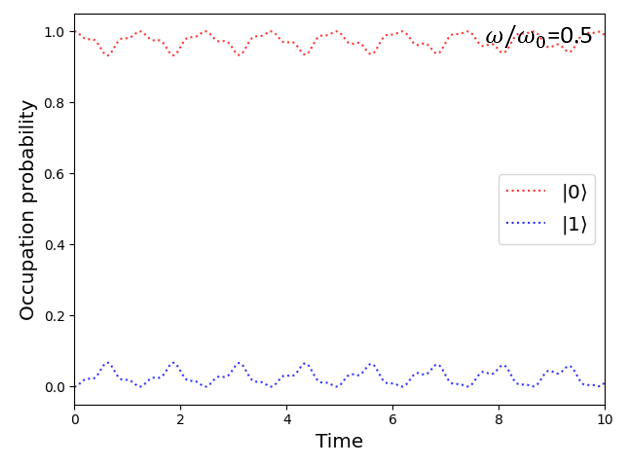
\includegraphics[scale=0.59]{F8}
\caption{Evolution of the state $|\psi\rangle$ in the two-level model. $\Omega_0 = 1$ and $|\psi(0)\rangle = |0\rangle$ in both evolutions.}
\end{figure}
From this figure, in the $\delta = 0$ case, we see that the Rabi flopping has a period $T=2\pi\Omega_0$. That is, we are able to drive the system from state $|0\rangle$ to state $|1\rangle$ by having the external field (that gives constant $\Omega = \that{\Omega} = \Omega_0$) sharply turned on at $t = 0$ and sharply shut off at $t = \pi \Omega_0$, and this field is called a $\pi$-pulse. If we sharply shut off the field at $t = 2\pi \Omega_0$, the field is called a $2\pi$-pulse instead, which drives the atom back to its original state at $t = 0$. 

\subsection{$\pi$-pulse and $2\pi$-pulse}
In practice, it is more reasonable to have the external field turned on and off smoothly. In fact, for the case where $\delta = 0$, $\Omega(t) = \that{\Omega}(t) = \Omega_0(t)$, it suffices to have the pulse area
\begin{align}
\Theta = \int_{-\infty}^\infty \Omega_0(t) \, dt
\end{align}
to be $\pi$ in order to obtain a $\pi$-pulse driving the atom from state $|0\rangle$ to state $|1\rangle$ (or from state $|1\rangle$ to state $|0\rangle$) \cite{Berman}. When $\Theta = 2\pi$, we have a $2\pi$-pulse instead. Therefore, $\Omega_0(t)$, which is directly proportional to the field amplitude, can be constructed in a form corresponding to smoothly turning on and off of the field, and obtain a $\pi$-pulse or a $2\pi$-pulse by controlling $\Theta$. 

\subsection{Rotating-wave approximation}
To motivate the discussion of Floquet theory in the second part of the text, we first introduce the rotating-wave approximation (RWA) in addressing the two-level system problems. In the interaction picture of the two-level system, $\that{H} = U^\dagger H U$, where $U = \exp(-iH_\text{a}t)$, thus we can write
\begin{align}
\that{H} =  \left(\Omega e^{i\delta t} + \that{\Omega} e^{i(\omega+ \omega_0) t}\right) |1\rangle\langle 0| + (\text{h.c.})\,.
\end{align} 
Whenever $|\that{\Omega}/(\omega_0+\omega)| \ll 1$ and $|\delta /(\omega_0+\omega)|\ll 1$, the rapidly oscillating terms
do not contribute much since they average to zero in a very short period of time. In other words, the contribution from these rapidly varying terms would be negligibly
small compared with the slowly varying terms if we take a coarse-grain time average over a time interval much greater than
$1/(\omega_0 + \omega)$. We therefore employ the rotating wave approximation (RWA), that is neglecting the counter-rotating terms in the Hamiltonian, whenever we have $|\that{\Omega}/(\omega_0+\omega)| \ll 1$ and $|\delta /(\omega_0+\omega)|\ll 1$.
Under RWA, the Hamiltonian in the original frame reads
\begin{align}
H_{\text{RWA}} = H_\text{a} +  \left(\Omega e^{-i\omega t}|1\rangle\langle 0| + \Omega^* e^{i\omega t}|0\rangle \langle 1|\right)\,.
\end{align}
The Hamiltonian described by Eq.\,(6) has been extensively studied, and there have been numerous researches demonstrating the Rabi oscillation characterized by $\Omega$ \cite{Dudin, Gentile, Shandarova}. 

\section{Rydberg CNOT Gate}

\subsection{Rydberg Blockade}
Another key component in building the Rydberg CNOT gate is the Rydberg blockade mechanism. As Rydberg atoms are excited atoms that are highly sensitive to the external field, when one brings two Rydberg atoms closed together, the two will strongly interact. Denote the ground state of the atom as $|0\rangle$ and the (excited) Rydberg  state of the atom as $|r\rangle$. The two-atom system then has states $|gg\rangle$, $|gr\rangle$, $|rg\rangle$, and $|rr\rangle$. The interaction between the atoms can be modeled by the Van der Waals interaction, and thus the dynamics of the system can be described by the Hamiltonian
\begin{align}
H &= \frac{\Omega}{2}(|g\rangle \langle r|\otimes \mathbb{I} + \mathbb{I}\otimes |g\rangle\langle r|  +(\text{h.c.})) - \frac{C_6}{R^6}|rr\rangle \langle rr|\,,\tag{11}
\end{align}
\setcounter{equation}{11}\\
where $C_6$ is the Van der Waals coefficient, and $R$ is the distance between the two atoms \cite{Hanover}. From the Hamiltonian it is clear to see that, in the regime of strong interaction, $|C_6|/R^6 \gg \Omega$, the $|rr\rangle\langle rr|$ term has no effect on the first excitation (using a suitable $\pi$-pulse) from the $|gg\rangle$ state to the $|rg\rangle$ (or $|gr\rangle$) state, but it makes the second excitation (using the same $\pi$-pulse as the first excitation) from the $|rg\rangle$ (or $|gr\rangle$) state to the $|rr\rangle$ state off-resonant. This result is called the Rydberg blockade and is used to construct the Rydberg CNOT gate. The distance at which the Rydberg blockade sets in can be determined by comparing the interaction strength $(C_6/R^6)$ to the Rabi frequency $\Omega$, and is called the Rydberg distance, 
\begin{align}
R_b = \left(\frac{|C_6|}{\Omega} \right)^{1/6}\,,
\end{align}
where in typical experiments, $R_b$ is on the order of $10\, \mu$m.

\subsection{The Rydberg AS CNOT gate}
Now we have the key ingredients to understand the working mechanism of the Rydberg CNOT gate: (1) On- and off-resonance between the field frequency and the separation between two levels of an atom affect the driving between the levels; (2) The Rydberg blockade shifts the energy level of the $|rr\rangle$ state. We review here the protocol of the AS CNOT gate (controlled amplitude SWAP) built with Rydberg atoms presented in Ref.\,\cite{Isenhower}. In their work, they also have proposed the H-C$_\text{z}$ CNOT gate (Hadamard-C$_\text{z}$) which also utilizes the two main ingredients as mentioned.\\

The protocol of the AS CNOT gate proceeds as follows and is illustrated in Fig.\,2. 
\begin{figure}
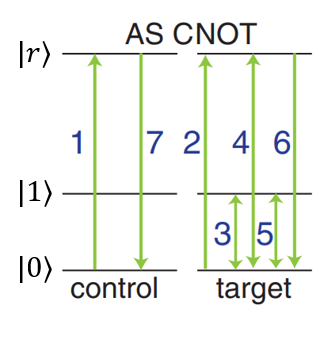
\includegraphics[scale=0.5]{F6}
\caption{The Rydberg AS CNOT gate protocol, taken from Fig.\,1 in Ref.\,\cite{Isenhower}. All arrows indicate $\pi$-pulse drivings, with the order of implementation indicated by the numbers.}
\end{figure}
Two atoms are prepared and are brought closed together with a separation distance around $10\,\mu$m, each has states $|0\rangle_q$, $|1\rangle_q$, and a Rydberg state $|r\rangle_q$ (with $q$ being $c$ for control qubit and $t$ for target qubit). One atom serves as the control qubit, and the other serves as the target qubit. All pulses used are $\pi$-pulses with suitable frequencies driving between states. First we apply a pulse on control driving between $|0\rangle_c$ and $|r\rangle_c$. Then we apply a pulse on target driving between $|0\rangle_t$ and $|r\rangle_t$, so if the control qubit is initially at $|0\rangle_c$, this pulse will fail to drive $|0\rangle_t$ to $|r\rangle_t$ due to Rydberg blockade. The third pulse drives target between $|0\rangle_t$ and $|1\rangle_t$. The fourth pulse drives target between $|r\rangle_t$ and $|0\rangle_t$, which will again fail if the initial state of control is $|0\rangle_c$. The fifth pulse drive target between $|0\rangle_t$ and $|1\rangle_t$. The sixth pulse drives target between $|r\rangle_t$ and $|0\rangle_t$, where Rydberg blockade might again set in. The last pulse drives control between $|r\rangle_c$ and $|0\rangle_c$. We see that the control qubit remains in $|0\rangle_c$ or $|1\rangle_c$ after the pulses, up to a single-qubit phase difference. On the other hand, if the control qubit is initially at $|0\rangle_c$, the second, fourth, and sixth pulses fail due to Rydberg blockade, and thus the target qubit undergoes a $2\pi$-pulse going back to its original state, up to a single-qubit phase difference. If the control qubit is initially at $|1\rangle_c$, following the protocol one can easily verify that the target qubit flips between $|0\rangle_t$ and $|1\rangle_t$. Thus this protocal corresponds to the standard CNOT gate apart from single qubit phase differences that can be corrected.\\

The experimental implementation of the AS CNOT gate involves using $^{87}$Rb atoms localized in far off-resonant traps, having measure temperature of around $200\,\mu$K, and being separated by around $10\,\mu$m. From here we see that the advantages of utilizing Rydberg atoms in realizing CNOT gate experimentally are: (1) It can be operated on micro-second time scales after taking the consideration of the lifetime of the Rydberg state of the atoms; (2) It does not require precise control of the two-atom interaction strength as long as Rydberg blockade sets in; (3) It is not limited to nearest neighbor interactions which is advantageous for scaling to multiqubit systems. However, as reported in Ref.\,\cite{Isenhower}, the fidelity of the gate is only around $0.73$, which is yet to be improved.\\

The experimental realization of the Rabi flopping between the ground state and the Rydberg state of $^{87}$Rb and the Rydberg blockade phenomena are presented in Ref.\,\cite{Urban} in 2009. The experimental implementation of the AS CNOT gate is presented in Ref.\,\cite{Isenhower} in 2010. In recent years, more progress on neutral atom quantum computation has been made, Ref.\,\cite{Saffman} has summarizes highlights and challenges in this field in 2016. This concludes the first part of the text. 


\section{\label{sec:level1}The Floquet Theory}
Having discussed the working mechanism of the Rydberg CNOT gate, it is not difficult to see the important role played by the two-level system model in studying quantum optics. In the second part of this text, we investigate the application of the Floquet theory in two-level systems, which makes use of the time periodicity in the Hamiltonian and thus help solving the time evolution of a state in a great extend. 


\subsection{Quasi-energies and Floquet Modes}
The Floquet's Theorem asserts that a collection of time-dependent differential equations, where the coefficients vary periodically with respect to time, will yield solutions that exhibit identical periodicity. This is a temporal analog of Bloch's theorem in spatial contexts, with solutions described in quasi-energies rather than quasi-momenta. We will first introduce the Floquet modes and quasi-energies, then we will compare them to their spatial analog from the Bloch's Theorem.\\

We first consider the time-dependent Schrodinger equation
\begin{align}
i \frac{d}{dt}|\psi(t)\rangle = H(t) \, |\psi(t)\rangle\,,
\end{align} 
for a periodic Hamiltonian 
\begin{align}
H(t) = H(t+nT)
\end{align}
for all $n \in \mathbb{Z}$. Via the Floquet Theorem, a solution $|\psi_\alpha(t)\rangle$ to Eq.\,(7) can be written as,
\begin{align}
|\psi_\alpha(t)\rangle =  e^{-i \epsilon_\alpha t }|\phi_\alpha (t)\rangle\,,
\end{align}
where $|\phi_\alpha(t) \rangle = |\phi_\alpha(t+nT)\rangle$ is called a Floquet mode, the time-independent quantity $\epsilon_\alpha$ is called the associated quasi-energies, uniquely defined up to multiples of $\omega = 2\pi/T$, and $|\psi_\alpha(t)\rangle$ is called a Floquet state. A general solution to Eq.\,(7) can be written as a linear combination of the Floquet state $|\phi_\alpha(t)\rangle$. Now we define
\begin{align}
G(t) = H(t) - i \frac{d}{dt}\,,
\end{align}
and combining Eq.\,(9) with Eq.\,(7), we obtain the eigenvalue problem that we are interested in solving,
\begin{align}
G(t) \, |\phi_\alpha (t) \rangle = \epsilon_\alpha |\phi_\alpha(t)\rangle\,,
\end{align}
with $G$ called the quasi-energy operator. That is, to find the Floquet modes and quasi-energies, we solve Eq.\,(10) numerically, or even analytically. \\

\subsection{Comparison with the Bloch Theory}
To gain more insights into the definition of Floquet modes and quasi-energies, we first have a review of the spatial analog of the Floquet theory, the Bloch theory. In this case, we consider the time-independent Schrodinger equation for a Hamiltonian with a spatially periodic potential $V(x) = V(x+a)$, where $a$ is the lattice spacing. Bloch's Theorem suggests that the solution to the time-independent Schrodinger's equation has the form
\begin{align}
|\psi (x,q) \rangle = u(x,q) \cdot e^{iqx}\,,
\end{align}
where $u(x,q)$ is called the Bloch function and has the same periodicity as the potential, $\psi(x,q)$ is called the Bloch wave, and $q$ is called
quasi-momentum or lattice momentum. We see immediately that Eq.\,(9) from the Floquet theory is of a form closely related to Eq.\,(12) from the Bloch theory, hence the name of quasi-energy for $\epsilon_\alpha$, and Floquet modes for $|\phi_\alpha (t)\rangle$. It seems that, in either Floquet theory or Bloch theory, we merely transform the problem from finding the unknown states $|\psi(t)\rangle$ or $|\psi(x,q)\rangle$ to finding the unknown states $|\phi_\alpha(t)\rangle$ or $u(x,q)$, but the crucial advantage is the periodicity in $|\phi_\alpha(t)\rangle$ and $u(x,q)$, which allows for Fourier transformation on those functionals. In Bloch theory, we can expand
\begin{align}
u(x,q) = \sum_{l} c_l(q)\, e^{iklx}\,,
\end{align}
where $q\,\text{mod}\,2k = 2\pi/a$, and thus we can write
\begin{align}
\psi(x,q) = \sum_l c_l(q)\, e^{i(2kl+q)x}\,,
\end{align}
which allows us to rewrite the corresponding Hamiltonian in the basis of plane waves. Similarly, for the Floquet theory model, we can expand
\begin{align}
|\phi_\alpha(t)\rangle = \sum_n e^{-i\omega n t} |\alpha, n\rangle\,,
\end{align}
and decompose the Hamiltonian 
\begin{align}
H(t) = \sum_n e^{i\omega n t} H_n\,,
\end{align}
where we define the Fourier components $|\alpha, n\rangle$ and $H_n$ via the usual way,
\begin{align}
|\alpha, n\rangle = \frac{1}{T}\int_0^T \, dt \, e^{i\omega n t}|\phi_\alpha(t)\rangle\,,
\end{align}
and 
\begin{align}
H_n =\frac{1}{T}\int_0^T\, dt\,
e^{i\omega n t}H(t)\,. 
\end{align}
This enables us to transform the open boundary condition problem characterized by Eq.\,(7) into a periodic boundary condition problem. In this sense, one can define the Floquet Hamiltonian $H_{\text{F}}$ to be the periodic-time-averaged of the quasi-energy operator, which has a matrix representation in the basis of the Fourier components, with entry $\langle \alpha, m |H_{\text{F}}|\beta, n\rangle$ given by
\begin{align}
\frac{1}{T}\int_0^Tdt\, \langle \alpha, m | H_{\text{F}} | \beta, n\rangle  = \langle \alpha | H_{m-n} | \beta \rangle + \delta_{m,n}\delta_{\alpha,\beta}m \omega\,.
\end{align}
\subsection{Time Evolution Operator}
Furthermore, we can consider the propagator $U(T+t,t)$ for the time-dependent Schrodinger equation Eq.\,(7), defined by 
\begin{align}
U(T+t,t)|\psi(t)\rangle = |\psi(T+t)\rangle\,.
\end{align}
Using the periodicity of $|\Phi_\alpha(t)\rangle$, we can write
\begin{align}
U(nT+t,t)\, |\phi_\alpha(t)\rangle = e^{-i\epsilon_\alpha T}|\phi_\alpha(t)\rangle = \eta_\alpha |\phi_\alpha(t)\rangle\,,
\end{align}
which suggests that the Floquet modes are eigenmodes of the multiple-period propagator, and we can therefore find the Floquet modes and quasienergies $\epsilon_\alpha = -\text{arg}(\eta_\alpha)/T$ by numerically calculating $U(nT+t,t)$ and diagonalizing it. This process can be first done to $U(T,0)$ to find $|\phi_\alpha(0)\rangle$ and the quasi-energies, then by employing Eq.\,(9), (19) and (20), one can directly evaluate $|\phi_\alpha(t)\rangle$, $|\psi_\alpha(t)\rangle$ and the general solution $|\psi(t)\rangle$ as a superposition of $|\psi_\alpha(t)\rangle$ at any other time $t$, with coefficients $c_\alpha$ determined by the initial wavefunction 
\begin{align}
|\psi(0)\rangle = \sum_\alpha c_\alpha |\psi_\alpha(0)\rangle\,.
\end{align}

This method is utilized by the Python library QuTiP to numerically compute the solution to the time-dependent Schrodinger equation \cite{QuTiP}, and is used to compute the evolution of a state presented in Section V.

\subsection{The Extended Hilbert Space}
Finally, we discuss a method of obtaining the quasi-energies by extending the Hilbert space. Using Eq.\,(15), it can be easily seen that 
\begin{align}
(\epsilon_\alpha + n \omega) | \alpha, n\rangle = \sum_{k} H_{n-k}|\alpha, k\rangle\,,
\end{align}
where $H_{l}$ for $l \in \mathbb{Z}$ is again the Fourier components of the Hamiltonian $H$. We see that we have created an over-complete problem as $\epsilon_\alpha$ are only defined up to multiples of $\omega$, and Eq.\,(23) can be recast into 
\begin{align}
\mathbf{M} \mathbf{v}_\alpha = \epsilon_\alpha \mathbf{v}_\alpha
\end{align}
where $\mathbf{M}$ is a matrix
\begin{align}
\mathbf{M} = \begin{pmatrix}
\ddots & H_{-1} & H_{-2} & \ddots \\
H_1 & H_0 -n\omega & H_{-1} & H_{-2} \\
H_2 & H_1 & H_0-(n+1) \hbar \omega & H_{-1}\\
\ddots & H_2 & H_1 & \ddots
\end{pmatrix}
\,, 
\end{align}
and $\mathbf{v}$ is a vector
\begin{align}
\mathbf{v}_\alpha = 
\begin{pmatrix}
\vdots\\
|\alpha, n\rangle \\
|\alpha, n+1\rangle\\
\vdots
\end{pmatrix}\,.
\end{align}
Note that $\mathbf{M}$ consists of blocks of $d\times d$ entries where $d$ is the dimension of the Hilbert space of $H$, and likewise, $|\alpha, n\rangle$ is $d$-dimensional.\\

A common time-dependent Hamiltonian, such as the one defined by Eq.\,(2) describing a qubit interacting with an external field, has the form
\begin{align}
H(t) = H_0 + Ve^{i\omega t} + V^\dagger e^{-i\omega t}\,,
\end{align}
in which case $\mathbf{M}$ takes the form
\begin{align}
\mathbf{M} = 
\begin{pmatrix}
\ddots & V & 0 & 0& \ddots \\
V^\dagger & H_0 +\omega & V & 0 & 0 \\
0& V^\dagger & H_0 & V&0\\
0 & 0 & V^\dagger & H_0 - \omega & V \\
\ddots & 0 & 0 & V^\dagger &\ddots
\end{pmatrix}
\,, 
\end{align}
which is similar to a tight-binding Hamiltonian with the nearest-neighbor hopping. \\

For the system described by Eq.\,(2) with $\that{\Omega} = \Omega^*$, Eq.\,(27) captures the full picture of the system, and thus the numerical evaluation of the Eq.\,(28) can be very efficient. In general, to truncate the evaluation of Eq.\,(28), it is crucial to distinguish two regimes. In the weak driving regime ($\omega\gg \langle V\rangle$), only one block 
\begin{align*}
\begin{pmatrix}
H_0+\omega & V \\ V^\dagger& H_0
\end{pmatrix}
\end{align*}
is relevant. When $\omega \sim \langle V\rangle$, which is the strong-driving limit, more blocks of matrix $\mathbf{M}$ shall be taken into account \cite{Viebahn}. 

\section{Application in Studying Two-level Systems}
Here we consider the two-level system described by the Hamiltonian defined in Eq.\,(2), (3), and (4). We first obtain the evolution of a state, for instance, $|\psi(0)\rangle =  |0\rangle$, using the Floquet theory and the time evolution operator. The method is entailed in part C of Section IV. With $\omega_0 = 10$, $\omega = 9$, and $\Omega =\that{\Omega} = 1$, the computed occupation probability for states $|1\rangle$ and $|0\rangle$ are plotted using dashed curves in Fig.\,3(a). Then we compute the evolution of the same state, $|\psi(0)\rangle =  |0\rangle$, by numerically solving the time-dependent Schrodinger equation, Eq.\,(7), with the result computed with RWA plotted in dotted curves in Fig.\,3(a), and the result computed without RWA plotted in solid curves. It is easy to see that all three methods agree quite well in this case as the conditions of using RWA are satisfied. We perform the same computations but with parameters $\omega_0 = 10$, $\omega = 9$, and $\Omega= \that{\Omega} = 10$, with results depicted in Fig.\,3(b). In this case, $|\that{\Omega}/(\omega_0+\omega)| \ll 1$ does not hold and thus RWA shall not be employed. Indeed, we see that the result computed via the Floquet theory agrees with the result obtained by numerically solving Eq.\,(7) without RWA, and they disagree with the result computed with RWA. Lastly, Fig.\,3(c) depicts the computations with $\omega_0 = 10$, $\omega = 3$, and $\Omega= \that{\Omega} = 1$, where RWA is again not applicable. \\

\begin{figure}
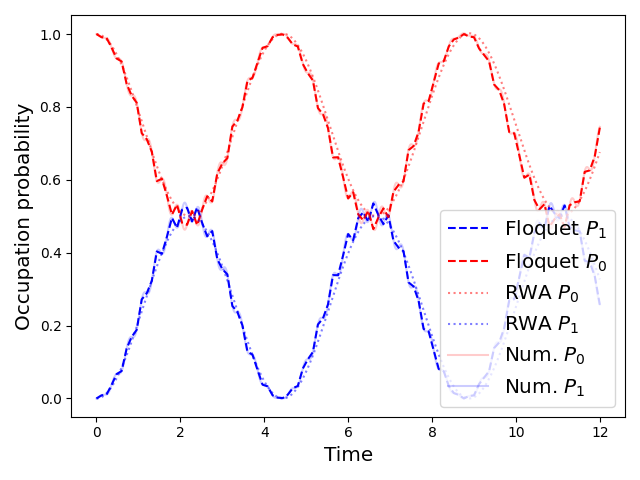
\includegraphics[scale=0.46]{F1}
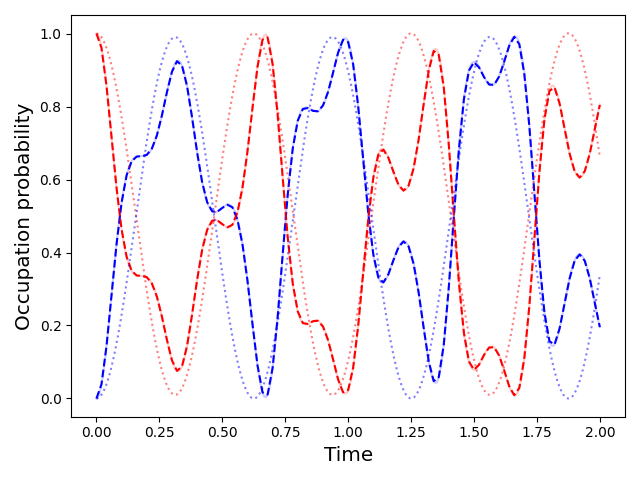
\includegraphics[scale=0.46]{F2}
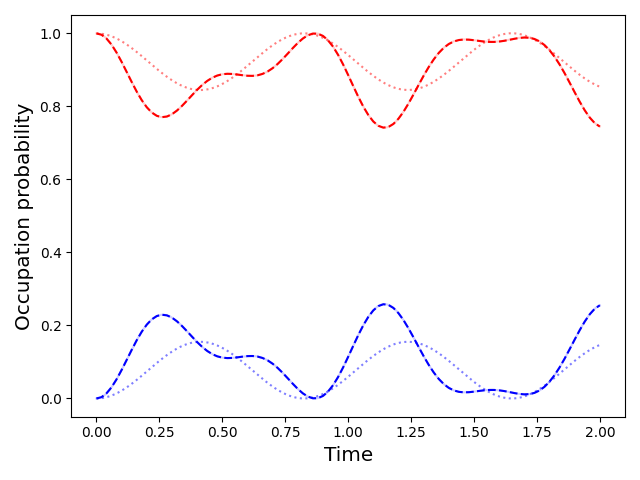
\includegraphics[scale=0.46]{F4}
\caption{The evolution of state $|\psi(0)\rangle = |0\rangle$, computed using three different methods: Using the time evolution operator with the Floquet theory, entailed in part C of Section IV; Numerically solving Eq.\,(7) without RWA; Numerically solving Eq.\,(7) with RWA. Note $\omega_0 = 10$ in all three computations. Subplot (a) is computed with $\Omega =\that{\Omega} = 1$ and $\omega = 9$, (b) is computed with $\Omega =\that{\Omega} = 10$ and $\omega = 9$, and (c) is computed with $\Omega = \that{\Omega }=1$ and $\omega = 3$.}
\end{figure}

We note that one advantage of employing the Floquet theory is that it requires less computational cost than numerically solving the time-dependent Schrodinger equation. This is because we can exploit the periodicity in the problem: To determine the evolution of a state $|\psi(t)\rangle$
at any time $t$,
we only need to compute $\epsilon_\alpha$ and the states $|\phi_\alpha(0)\rangle$ at $t = 0$, and the states
\begin{align}
|\phi_\alpha(\tau+nT)\rangle=|\phi_\alpha(\tau)\rangle = e^{i\epsilon_\alpha \tau} U(\tau,0) |\phi_\alpha(0)\rangle 
\end{align}
in the Brillouin zone $\tau \in [0,T]$. Then $|\psi(t)\rangle$ can be computed via the superposition
\begin{align}
|\psi(t)\rangle = \sum_\alpha c_\alpha e^{-i\epsilon_\alpha t}|\phi_\alpha(t)\rangle\,,
\end{align}
with the time-independent coefficients $c_\alpha$ determined by the initial state at time $t = 0$. Whereas numerically solving Eq.\,(7) requires fine time steps, and thus the computation cost for evaluating $|\psi(t)\rangle$ at a later time $t\gg T$ is much larger. Moreover, if there is no analytic solution available and without the application of Floquet theory, it is difficult to look up the evolution of the state at an arbitrary time $t_0$ without numerically solving the state at all time $t<t_0$, while the application of Floquet theory can be used to efficiently lookup the Floquet mode at an arbitrary time and thus constructing the state at an arbitrary time. \\

On the other hand, interesting observations can also be drawn from the quasi-energy of the system. Again, with $\omega = 9$ and $\omega_0= 10$, the quasi-energies of the system as a function of $\Omega/ \omega$ can be computed, shown in Fig.\,4. 
\begin{figure}
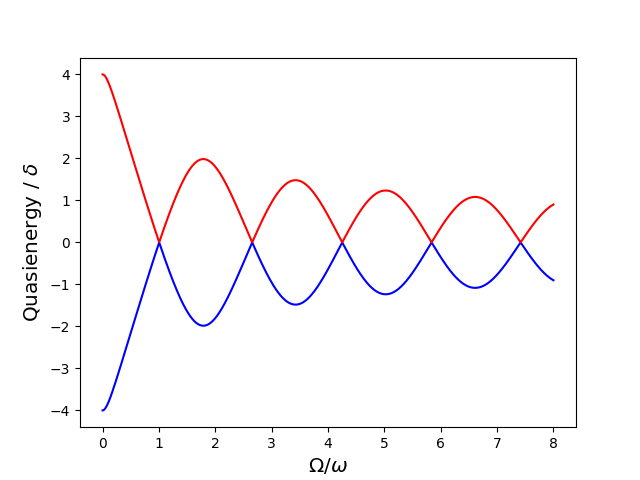
\includegraphics[scale=0.45]{F3}
\caption{Quasi-energy of the system as a function of $\Omega/\omega $ with $\omega = 9$ and $\omega_0= 10$. }
\end{figure}
We observe that the quasi-energies cross at certain values of $\Omega/ \omega$. These points are closely related to the coherent destruction of tunneling and have been shown to exhibit interesting phenomena \cite{QuTiP, Grossmann, Miao, Kayanuma}. \\


Other than the application in the semi-classical approach of describing the atom interacting with a driving field, the Floquet theory can also be applied in studying the Jaynes-Cummings model (JCM) \cite{Engelhardt, Wang, Ermann}. Many works have focused on studying the JCM with RWA applied. With the counter-rotating terms included, a general treatment to study the JCM is again by applying the Floquet theory. In the Schrodinger picture, the total Hamiltonian of the JCM reads
\begin{align}
H = H_0 + H_{\text{int}}
\end{align}
where 
\begin{align}
H_0 = \frac{\omega_0}{2}\sigma_z + \omega\hat{a}^\dagger \hat{a}
\end{align}
is the bare Hamiltonian of the atom and the field, and 
\begin{align}
H_{\text{int}} = g(\hat{a}+ \hat{a}^\dagger) (\sigma_+ + \sigma_-)
\end{align}
is the interaction Hamiltonian. Turning to the interaction picture, a frame rotating with frequency $\omega_0$, the Hamiltonian in Eq.\,(25) reads
\begin{align}
\that{H} = \frac{\delta}{2}\sigma_z + g(\hat{a}\sigma_+ + \hat{a}^\dagger \sigma_-) + g(\hat{a}\sigma_- e^{-2i\omega t} + \hat{a}\sigma_+ e^{2i\omega t})\,,
\end{align}
where $\delta = \omega_0 - \omega$ is again the atom-light detuning. We notice that the Hamiltonian $\that{H}$ is periodic with frequency $2\omega$, thus Floquet theory can be applied. We can decompose Eq.\,(28) into its Fourier components,
\begin{align}
H = H_0 + H_1 e^{i2\omega t} + H_{-1}e^{-i2\omega t}\,,
\end{align}
where we have
\begin{align}
H_0 &= g(\hat{a}\sigma_+ + \hat{a}^\dagger \sigma_- ) + \delta {\sigma_z}/{2}\,,\\
H_1 &= g \hat{a}^\dagger \sigma_+\,,\\
H_{-1} &= g\hat{a}\sigma_-\,.
\end{align}
Via the Floquet theory, the long-time evolution of Eq.\,(29) can be described by an effective time-independent Floquet Hamiltonian, 
\begin{align}
H_{\text{F,\,eff}} = \sum_{n=0}^\infty \frac{1}{(2\omega)^n}H^{(n)} \approx H^{(0)} + \frac{1}{2\omega}H^{(1)} + \frac{1}{4\omega^2} H^{(2)}\,,
\end{align}
with $H^{(0)} = H_0$, 
\begin{align}
H^{(1)} =[H_1,H_{-1}] = \frac{g^2}{2}\left( (2\hat{n} + 1) \sigma_z - \sigma_z^2\right)\,,
\end{align}
and 
\begin{align*}
H^{(2)} &= \frac{1}{2}\left( [[H_1,H_0], H_{-1}] + [[H_{-1},H_0], H_1]\right)\\
&=-\frac{\delta g^2}{2}\left( (2\hat{n}+1) \sigma_z - \sigma_z^2\right) - g^3\left( \hat{a}\sigma_+ \hat{n} + \hat{n}\hat{a}^\dagger \sigma_0\right)\,. \tag{36}
\end{align*}
Combining and grouping terms, we obtain a high-frequency effective Hamiltonian,
\begin{align}
H_{\text{F,\,eff}} \approx 
\frac{\that{\delta}_{\omega, \hat{n}}}{2} \sigma_z + \left( \hat{g}_{\omega, \hat{n}} \sigma_- + (\text{h.c.})\right) + \frac{\delta_{\omega}}{2}\,,
\end{align}
with coefficients defined by
\begin{align}
\that{\delta}_{\omega, \hat{n}} &=
\left(1- (2\hat{n}+1)\frac{g^2}{4\omega^2} \right)\delta + (2\hat{n}+1) \frac{g^2}{2\omega}\,, \\
\that{g}_{\omega, \hat{n}} &= \left(1 - \frac{g^2}{4\omega^2}\hat{n}  \right)g\,,\\
\delta_{\omega} &= -\frac{g^2}{2\omega} + \frac{g^2\delta}{4\omega^2}\,.
\end{align}
Comparing Eq.\,(35) with the Hamiltonian of JCM in RWA, one sees that the counter-rotating terms have effects on the effective detuning $\that{\delta}_{\omega, \hat{n}}$ and the atom-light coupling $\that{g}_{\omega, \hat{n}}$. A detailed analysis of Eq.\,(35) is given by Wang.\, et al. in Ref.\,\cite{Wang}.\\

More studies on the JCM with the application of the Floquet theory include JCM under monochromatic driving by Ermann et al. \cite{Ermann}, the generation of light-matter entanglement, and the application of photon-resolved Floquet theory in quantum communication by Engelhardt et al. \cite{Engelhardt}, and so on. These results demonstrate that the Floquet theory can be used to effectively study the two-level system, especially in the regime of strong driving, and strong matter-photon coupling. \\


\section{Optical Lattices with Floquet Engineering}
One of the primary areas of research garnering significant attention lately is the Floquet engineering in optical lattices \cite{Sandholzer, Subhankar, Wu, Sandholzer2}. This field combines Bloch theory, which describes spatial periodicity in potential, with Floquet theory, which characterizes temporal periodicity in potential, resulting in the emergence of Floquet-Bloch waves.\\

An intriguing effect brought by Floquet engineering that has captured people's interest is the shaking of optical lattices, which has been shown to manifest fascinating topological phenomena  \cite{12n, 16,17,18,19} and has become an important tool for controlling and manipulating cold atom systems \cite{15,24,25}. In this section, we present the theoretical framework for describing optical lattice shaking. \\

\begin{figure}
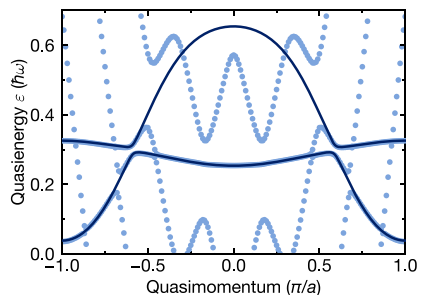
\includegraphics[scale=0.85]{F5}
\caption{Floquet-Bloch bands, taken from Fig.\,7 in \cite{Sandholzer}. The dispersion of the effective two-band Hamiltonians (solid lines) is compared to the numerical exact solution of the Floquet-Bloch band structure (points, three lowest bands). }
\end{figure}

In $1$-dimensional crystal lattice, a common experimental method in implementing lattice shaking employs a piezo-electric actuator \cite{Viebahn, Sandholzer}, which moves the retro-reflecting mirror that defines the standing wave, and thus the potential of the optical lattice $V$ is modulated by a position and time $x(t)$. Another approach involves modulating the frequency of one of the two beams that form the standing wave that traps the atom \cite{Viebahn}. Thus, in either case, the Hamiltonian describing the system takes the form
\begin{align}
H_{\text{lab}}(t) = \frac{\hat{p}^2}{2m} + V(\hat{x} - x(t))\,
\end{align}
in the lab frame. It is possible to transform this Hamiltonian to the reference frame that is co-moving with the shaken lattice,
\begin{align}
H_{\text{cm}}(t) = \frac{\hat{p}^2}{2m} + V(\hat{x}) - F(t)\hat{x}\,,
\end{align}
where we have a time-periodic force $F(t)$ that shakes the lattice, and a spatial-periodic potential $V(\hat{x})$ responsible for trapping the atom. As Eq.\,(46) is periodic in space and time, Bloch and Floquet theory can be applied to study the system. As an example, the Floquet-Bloch bands in this type of system are shown in Fig.\,5, attributed to the work by Kilian Sandholzer et al. on the \textit{Floquet engineering of individual band gaps in an optical lattice using a two-tone drive} \cite{Sandholzer}. We note that the von Neumann–Wigner noncrossing rule leads to the formation of a band gap in quasimomentum when considering the single harmonic driving as the case depicted in Fig.\,5 \cite{57}. This results in the hybridization of the lowest band and the first excited band. In their work, the potential $V$ in the lab frame takes the form
\begin{align}
V = -V_X \cos^2\left( k_L \hat{x} - k_L x_0(\tau)\right)\,,
\end{align}
where the depth $V_X$ and the phase $k_Lx_0$ are controlled by varying the intensity of the laser and the position of the retroreflecting mirror. They use a piezoelectric actuator to obtain precise and fast control of the mirror position defining the phase of the lattice potential 
\begin{align}
k_Lx_0(\tau) = \frac{2E_{\text{rec}}}{\pi \hbar \omega}\left( K_\omega \cos(\omega \tau) + \frac{K_{l\omega}}{l}\cos(l\omega \tau +\phi)\right)\,,
\end{align}
where $E_{\text{rec}}$ is the recoil energy, $k_L$ is the wave vector of the lattice laser, and $K_\omega$ and $K_{l\omega}$ are the dimensionless driving strengths. Utilizing this setup, they experimentally and theoretically study two-frequency phase modulation to asymmetrically hybridize the lowest two bands of the one-dimensional lattice, and it is worth noticing that their theoretical framework in studying the model is based on that described by Eq.\,(28), turning a two-level-system problem into a tight-binding-model problem. 

\section{Summary}
In this text, we start by introducing the two-level system, the Rydberg blockade, and their application in constructing the Rydberg AS CNOT gate. Then in the second part of the text, we have demonstrated that the Floquet theory helps us in efficiently computing the state of the two-level system in the semi-classical approach by exploiting the time periodicity in the Hamiltonian. We have shown that the Floquet theory can turn a two-level problem into a tight-binding model in the extended Hilbert space. Moreover, Floquet theory can also be applied to study the Jaynes-Cummings model describing the two-level system, and we have investigated how the counter-rotating term plays a role in the evolution of the system in the Jaynes-Cummings model. Lastly, we have introduced Floquet engineering in optical lattice, based on the study by Sandholzer et al. on shaking optical lattice. \\


%\section{Appendixes}
%\nocite{*}

\bibliography{apssamp}% Produces the bibliography via BibTeX.
\begin{thebibliography}{9}
\bibitem{2}
C. Monroe, D. M. Meekhof, B. E. King, W. M. Itano, and D. J. Wineland,
Phys. Rev. Lett. \textbf{75}, 4714 (1995).
\bibitem{3}
F. Schmidt-Kaler, H. Häffner, M. Riebe, S. Gulde, G. P. T. Lancaster, T. Deuschle, C. Becher, C. F. Roos, J. Eschner, and R. Blatt, Nature \textbf{422}, 408 (2003).
\bibitem{4}
T. Yamamoto, Y. A. Pashkin, O. Astafiev, Y. Nakamura, and J. S. Tsai, Nature \textbf{425}, 941 (2003).
\bibitem{5}
J. H. Plantenberg, P. C. de Groot, C. J. P. M. Harmans, and J. E. Mooij, Nature \textbf{447}, 836 (2007).
\bibitem{6}
J. L. O'Brien, G. J. Pryde, A. G. White, T. C. Ralph, and D. Branning, 
Nature \textbf{426}, 264 (2003).
\bibitem{7}
T. B. Pittman, M. J. Fitch, B. C Jacobs, and J. D. Franson, Phys. Rev. A \textbf{68}, 032316 (2003).
\bibitem{8}
G. K. Brennen, C. M. Caves, P. S. Jessen, and J. H. Deutsch, Phys. Rev. Lett. \textbf{82}, 1060 (1999).
\bibitem{9}
D. Jaksch, H.-J. Briegel, J. I. Cirac, C. W. Gardiner, and P. Zoller, Phys. Rev. Lett. \textbf{82}, 1975 (1999).
\bibitem{10}
T. Pellizzari, S. A. Gardiner, J. I. Cirac, and P. Zoller, Phys. Rev. Lett. \textbf{75}, 3788 (1995).
\bibitem{11}
L. You and M. S. Chapman, Phys. Rev. A \textbf{62}, 052302 (2000).
\bibitem{12}
C. W. J. Mompart, C. Emary, M. Kindermann, and J. L. van Velsen, Phys. Rev. Lett. \textbf{90}, 147901 (2003).
\bibitem{13}
D. Jaksch, J. I. Cirac, P. Zoller, S. L. Rolston, R. Côté, and M. D. Lukin, Phys. Rev. Lett. \textbf{85}, 2208 (2000).
\bibitem{Isenhower}
L. Isenhower, E. Urban, X. L. Zhang, A. T. Gill, T. Henage, T. A. Johnson, T. G. Walker, and M. Saffman, Phys. Rev. Lett. 104, 010503 (2010).
\bibitem{IsenhowerThesis}
L. Isenhower, Demonstration of Rydberg Blockade and a Neutral Atom CNOT Gate, Ph.D. thesis, University of Wisconsin – Madison, 2010.
\bibitem{Shirley}
J. H. Shirley, Phys. Rev. \textbf{138}, B979 (1965). 
\bibitem{Engelhardt}
G. Engelhardt, S. Choudhury, and W. V. Liu, Phys. Rev. Res. \textbf{6}, 013116 (2024). 
\bibitem{Wang}
Y.-F. Wang H.-H. Yin, M.-Y. Yang, A.-C. Ji, and Q. Sun, Chin. Phys. B \textbf{30} 064204 (2021).
\bibitem{Campaioli}
F. Campaioli, J. H. Cole, H. Hapuarachchi, \textit{A Tutorial on Quantum Master Equations: Tips and tricks for quantum optics, quantum computing and beyond}, arXiv:2303.16449, 2023. 
\bibitem{Viebahn}
K. Viebahn, \textit{Introduction to Floquet theory}, Bounder School for Condensed Matter and Material Physics (2020).
\bibitem{Rechtsman}
M. C. Rechtsman, J. M. Zeuner, Y. Plotnik, Y. Lumer, D. Podolsky, F. Dreisow, S. Nolte, M. Segev, and A. Szameit, Nature \textbf{496}, 196 (2013).
\bibitem{88}
R. W. Bomantara and J. Gong, Phys. Rev. B \textbf{98}, 65421 (2018).
\bibitem{89}
S. Restrepo, J. Cerrillo, P. Strasberg, and G. Schaller, New J. Phys. \textbf{20}, 053063 (2018).
\bibitem{90}
B. Bartels and F. Mintert, Phys. Rev. A \textbf{88}, 052315 (2013).
\bibitem{91}
A. Castro, U. De Giovannini, S. A. Sato, H. Hubener, and A. Rubio, Phys. Rev. Res. \textbf{4}, 033213 (2022).
\bibitem{92}
D. V. Else, B. Bauer, and C. Nayak, Phys. Rev. Lett. \textbf{117}, 090402 (2016).
\bibitem{93}
K. Sacha and J. Zakrzewski, Rep. Prog. Phys. \textbf{81}, 016401 (2018).
\bibitem{Sandholzer}
K. Sandholzer , A.-S. Walter, J. Minguzzi, Z. Zhu, K. Viebahn , and T. Esslinger, Phys. Rev. Res. \textbf{4}, 013056 (2022). 
\bibitem{Anderson}
B. M. Anderson, L. W. Clark, J. Crawford, A. Glatz, I. S. Aranson, P. Scherpelz, L. Feng, C. Chin, and K. Levin, Phys. Rev. Lett. \textbf{118}, 220401 (2017). 
\bibitem{Berman}
P. R. Berman and V. S. Malinovsky, Principles of Laser Spectroscopy and Quantum Optics (Princeton University Press, Princeton, NJ, USA, 2011).
\bibitem{Hanover}
H. Weimer, Rydberg Atoms (lecture note on interacting Rydberg atoms, Leibniz University Hannover, Hanover, Germany, 2015).
\bibitem{Urban}
E. Urban, T. A. Johnson, T. Henage, L. Isenhower, D. D. Yavuz, T. G. Walker and M. Saffman, Nat. Phys. 5, 110 (2009).
\bibitem{Saffman}
M. Saffman, J. Phys. B: At. Mol. Opt. Phys. 49, 202001 (2016).
\bibitem{Dudin}
Y. O. Dudin, L. Li, F. Bariani, and A. Kuzmich, Nat. Phys. \textbf{8}, 790 (2012).
\bibitem{Gentile}
T. R. Gentile, B. J. Hughey, D. Kleppner, and T. W. Ducas, Phys. Rev. A \textbf{40}, 5103 (1989). 
\bibitem{Shandarova}
K. Shandarova, C. E. Ruter, and D. Kip, Phys. Rev. Lett. \textbf{102}, 123905 (2009).
\bibitem{QuTiP}
P.D. Nation, J.R. Johansson, A.J.G. Pitchford, C. Granade, and A.L. Grimsmo, \textit{QuTiP: Quantum Toolbox in Python. User Guide: Time Evolution and Quantum System Dynamics, Floquet Formalism}, 2017. 
\bibitem{Grossmann}
F. Grossmann, T. Dittrich, P. Jung, and P. Hanggi, Phys. Rev. Lett. \textbf{67}, 4 (1991).
\bibitem{Miao}
Q. Miao and Y. Zheng, Sci. Rep. \textbf{6}, 28959 (2016).
\bibitem{Kayanuma}
Y. Kayanuma and K. Saito, Phys. Rev. A \textbf{77}, 010101(R) (2008).
\bibitem{Ermann}
L. Ermann, G. G. Carlo, A. D. Chepelianskii, and D. L. Shepelyansky, Phys. Rev. A \textbf{102}, 033729 (2020).
\bibitem{Subhankar}
S. Subhankar, P. Bienias, P. Titum, T.-C. Tsui, Y. Wang, A. V. Gorshkov, S. L. Rolston, and J. V. Porto, New J. Phys. \textbf{21}, 113058 (2019). 
\bibitem{Wu}
S. Wu, W. Song, Z. Lin, C. Chen, S. Zhu, and T. Li, Opt. Express \textbf{30}, pp. 44983 (2022). 
\bibitem{Sandholzer2}
K. Sandholzer, \textit{Floquet Engineering of Ultracold Atoms in Optical Lattices}, Dr. sc. thesis, ETH Zurich, 2022.
\bibitem{12n}
M. S. Rudner and N. H. Lindner, Nat. Rev. Phys. \textbf{2}, 229 (2020).
\bibitem{16}
T. Kitagawa, E. Berg, M. Rudner, and E. Demler, Phys. Rev. B \textbf{82}, 235114 (2010).
\bibitem{17}
J. Cayssol, B. Dóra, F. Simon, and R. Moessner, Phys. Status Solidi \textbf{7}, 101 (2013).
\bibitem{18}
Á. Gómez-León and G. Platero, Phys. Rev. Lett. \textbf{110}, 200403 (2013).
\bibitem{19}
T. Oka and S. Kitamura, Annu. Rev. Condens. Matter Phys. \textbf{10}, 387 (2019).
\bibitem{15}
N. R. Cooper, J. Dalibard, and I. B. Spielman, Rev. Mod. Phys. \textbf{91}, 015005 (2019).
\bibitem{24}
N. Goldman, J. C. Budich, and P. Zoller,  Nat. Phys. \textbf{12}, 639 (2016).
\bibitem{25}
C. Weitenberg and J. Simonet, Nat. Phys. \textbf{17}, 1342 (2021).
\bibitem{57}
J. von Neumann and E. P. Wigner, Z. Phys. \textbf{30}, 467 (1929).
\end{thebibliography}



\end{document}
%
% ****** End of file apssamp.tex ******
